\documentclass[aspectratio=169, pdf, 8pt, unicode]{beamer}
\usepackage[american,russian]{babel}
\usepackage[default]{sourcesanspro}
\usepackage{float}
\usepackage{graphicx}
\usepackage{pgfplotstable}
\usepackage{caption}
\usepackage{amsmath}
\usepackage{amssymb}
\usepackage{setspace}
\usepackage{fancyvrb}

\DeclareCaptionLabelFormat{gostfigure}{Рисунок #2}
\captionsetup[table]{labelsep=endash,justification=justified,singlelinecheck=false,font=normalsize,skip=0pt} 
\captionsetup[figure]{labelformat=gostfigure,labelsep=endash,justification=centering,singlelinecheck=false,font=normalsize} 
\pgfplotsset{compat=1.9}

\mode<presentation> {
\usetheme{Madrid}
}

\setbeamerfont{institute}{size=\normalsize}
\setbeamertemplate{itemize/enumerate body begin}{\large}
\setbeamertemplate{itemize/enumerate subbody begin}{\tiny}

\title[Теория и практика многопоточного программирования]{Теория и практика многопоточного программирования\\ \vspace{0.5cm}Семинар 2}

\author{Неганов Алексей}

\institute[МФТИ]{
    Московский физико-технический институт (национальный исследовательский университет)\\
    Кафедра теоретической и прикладной информатики\\
}

\date{Москва 2020}

\setbeamertemplate{caption}[numbered]

\begin{document}

\begin{frame}
\titlepage
\end{frame}

\begin{frame}[fragile]
\frametitle{Процессы}
\begin{figure}[H]
      \centering
      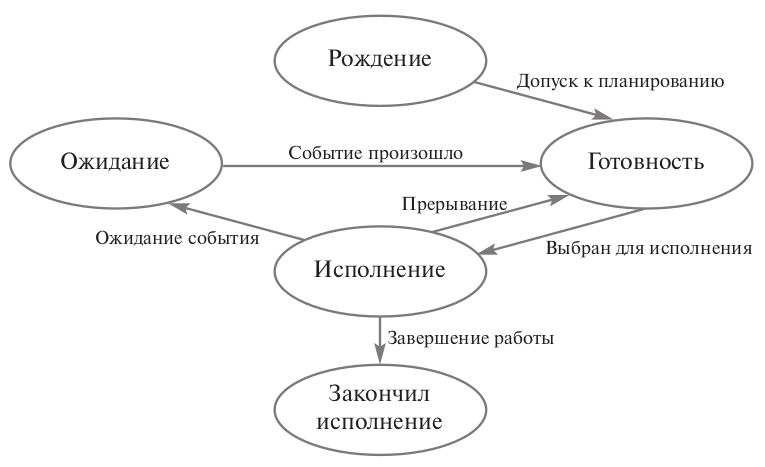
\includegraphics[width=0.7\textwidth]{fig/processes_diag.png}
      \caption{Упрощённая диаграмма состояний процесса}
\end{figure}
\end{frame}

\begin{frame}[fragile]
\frametitle{Процессы}
Что содержит процесс (пример UNIX):
	\begin{itemize}
		\item Сегмент кода (возможно, разделяемый) 
		\item Сегмент данных (включая стек)
		\item Состояние регистров, включая программный счётчик
		\item Таблица дескрипторов ввода-вывода
		\item Диспозиция обработки сигналов
		\item Счётчики потреблённых ресурсов
		\item Командная строка и окружение
		\item Текущий и корневой каталог
		\item Идентификаторы процесса, его родителя, группы и сеанса
		\item Информация о владельце
		\item Настройки прав
		\item ...
	\end{itemize}
\end{frame}

\begin{frame}[fragile]
\frametitle{Потоки (threads)}
Что содержит поток:
	\begin{itemize}
		\item Стек
		\item Состояние регистров, включая программный счётчик
	\end{itemize}
\begin{figure}[H]
      \centering
      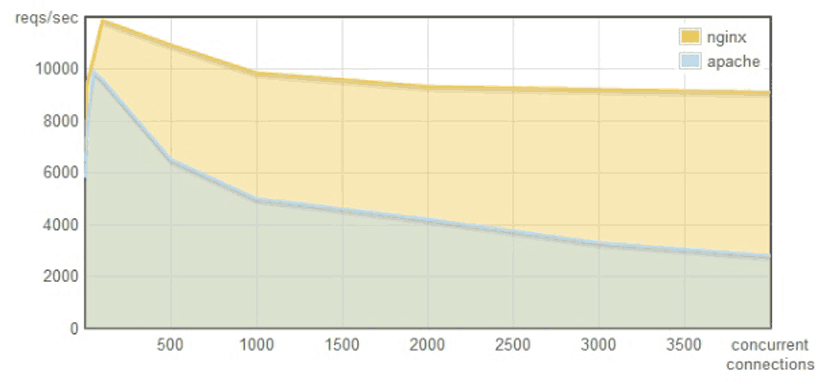
\includegraphics[width=0.6\textwidth]{fig/nginx-apache-10kreqs.png}
      \caption{Сравнение поведения веб-серверов Nginx и Apache при увеличении количества обновременных подключений}
\end{figure}
\end{frame}

\begin{frame}[fragile]
\frametitle{Сопрограммы}
\begin{figure}[H]
      \centering
		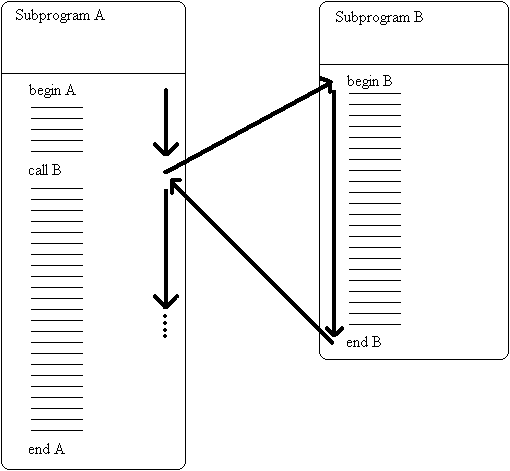
\includegraphics[width=0.4\textwidth]{fig/routine.png}
		\hspace{0.05\textwidth}
      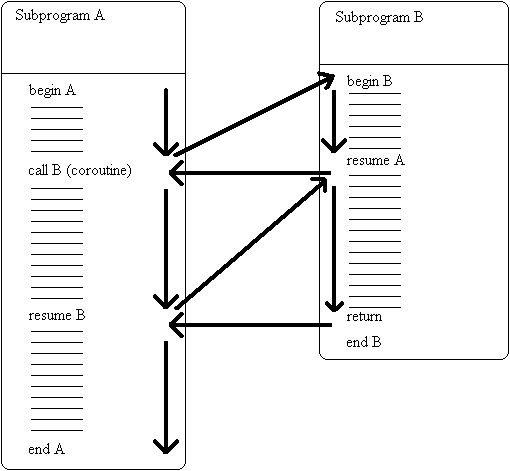
\includegraphics[width=0.4\textwidth]{fig/coroutine.png}
      \caption{Поток команд для программ и сопрограмм}
\end{figure}
\end{frame}

\begin{frame}[fragile]
\frametitle{Green threads / goroutines}
\begin{figure}[H]
      \centering
		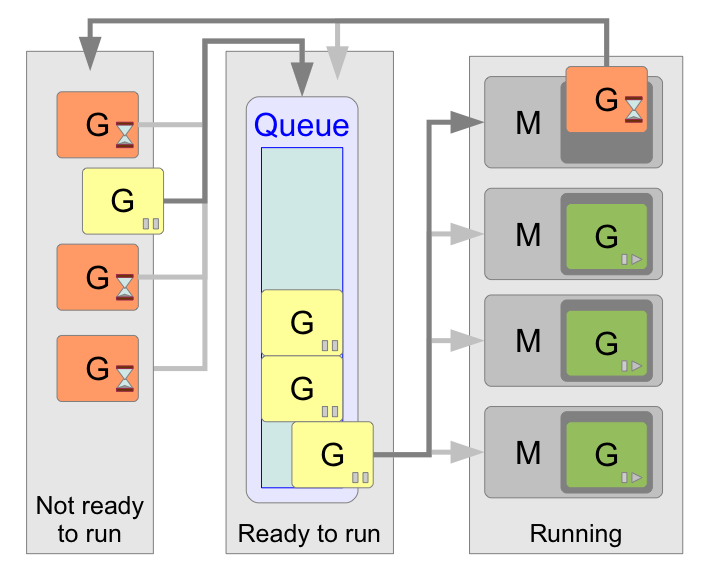
\includegraphics[width=0.55\textwidth]{fig/goroutines.png}
      \caption{Схема работы планировщика Go}
\end{figure}
\end{frame}


\begin{frame}
\frametitle{Гонки и критические секции}
\begin{block}{Ситуация гонок}
	Ситуацией гонок \textit{(race condition)} называется недетерминированность совокупного исполнения потоков.
\end{block}
\begin{block}{Критерий Бернстайна}
	Пусть $R(P_i)$ множество переменных, значение которых поток $P_i$ использует в операциях чтения, $W(P_i)$ ---
	множество переменных, использующихся в операциях записи. Тогда совокупное исполнение потоков $P_1$ и $P_2$ детерминировано, если
	\begin{equation}
	\left\{
	\begin{aligned}
		W(P_1) \cap W(P_2) = \varnothing \\
		R(P1)  \cap W(P_2) = \varnothing \\
		W(P_1) \cap R(P_2) = \varnothing \\
	\end{aligned}
	\right.
   \end{equation}
\end{block}
\end{frame}

\begin{frame}
\frametitle{Условия на код}
\begin{enumerate}
\item Два и более потока не должны ни при каких условиях находиться одновременно в критических секциях, связанных с одними и теми же данными
		\textit{(mutual exclusion)}
\item Хотя бы один из конкурирующих потоков должен рано или поздно попасть в нужную ему критическую секцию \textit{(freedom from deadlock)}
\item Каждый поток должен рано или поздно попасть в критическую секцию \textit{(freedom from starvation)}
\item Полезная работа над данными критической секции должна доводиться до конца \textit{(freedom from livelock)}
\item Основное время поток должен провести в исполнении полезной работы, а не в ожидании блокированного ресурса \textit{(freedom from lock contention)}
\item Заблокированный поток не должен расходовать процессорное время (отсутствие активного ожидания)
\end{enumerate}
\end{frame}

\begin{frame}[fragile]
\frametitle{Условия на код}
Верно ли, что методы \texttt{lock12()} и \texttt{lock21()}, будучи вызванными из разных потоков,
рано или поздно завершат работу? Какое название имеет такое состояние программы?
\begin{figure}[H]
\centering
\begin{BVerbatim}
mutex_t m1, m2;

void lock12(void) {                     void lock21(void) {
      m1.lock();                              m2.lock();
      while (m2.locked()) {                   while (m1.locked()) {
            m1.unlock();                            m2.unlock();
            wait();                                 wait();
            m1.lock();                              m2.lock();
      }                                       }
      m2.lock();                              m1.lock();
}                                       }
\end{BVerbatim}
\end{figure}
\end{frame}

\begin{frame}
\frametitle{Необходимые и достаточные условия возникновения тупиков (deadlock)}
\begin{enumerate}
\item Условие взаимоисключения \textit{(mutual exclusion):} существует ресурс такой, что единовременно использовать его только один поток
\item Условие ожидания ресурсов \textit{(hold and wait):} потоки, уже захватившие ресурсы, могут захватывать другие ресурсы
\item Условие неперераспределяемости \textit{(no preemption):} ресурс не может быть принудительно забран у потока, только сам поток может освободить его
\item Условие кругового ожидания \textit{(circular wait):} cуществует кольцевая цепь потоков, в которой каждый поток ждет доступа к ресурсу, удерживаемому другим потоком цепи
\end{enumerate}
\end{frame}

\begin{frame}
\frametitle{Необходимые и достаточные условия возникновения тупиков (deadlock)}
\begin{figure}[H]
      \centering
		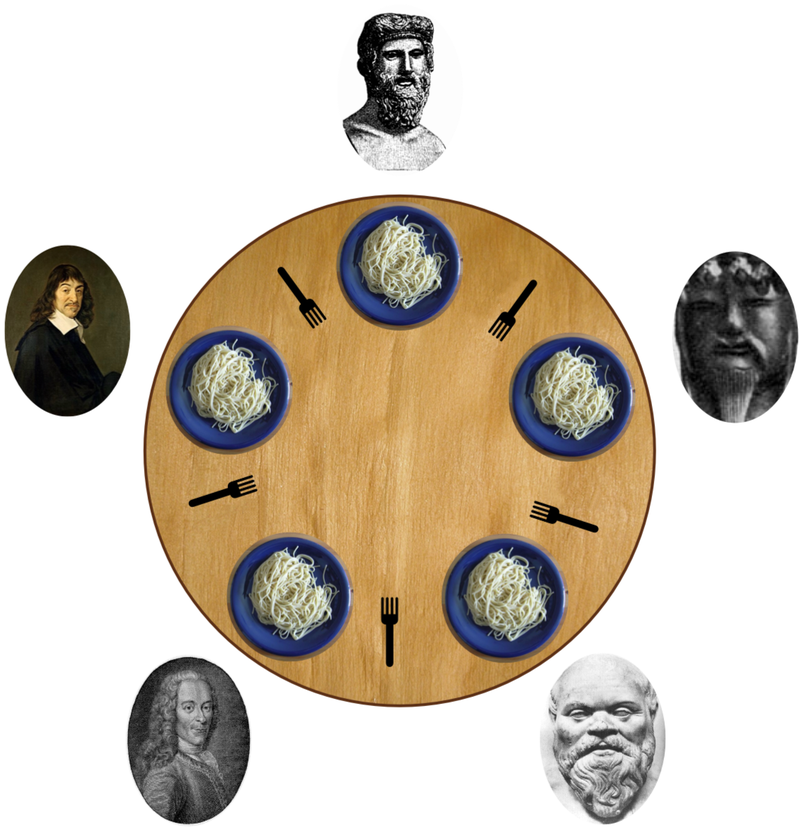
\includegraphics[width=0.4\textwidth]{fig/dining_philosophers_problem.png}
      \caption{Задача об обедающих философах}
\end{figure}
\end{frame}

\begin{frame}[fragile]
\frametitle{Необходимые и достаточные условия возникновения тупиков (deadlock)}
Рассмотрим псевдокод следующей программы, использующей семафоры:
\begin{figure}[H]
\centering
\begin{BVerbatim}
int x = 0, y = 0, z = 0;
sem lock1 = 1, lock2 = 1;

process foo {             process bar {
      z = z + 2;                P(lock2);
      P(lock1);                 y = y + 1;
      x = x + 2;                P(lock1);
      P(lock2);                 x = x + 1;
      V(lock1);                 V(lock1);
      y = y + 2;                V(lock2);
      V(lock2);                 z = z + 1;
}                         }
\end{BVerbatim}
\end{figure}
Может ли эта программа войти в состояние взаимной блокировки \textit{(deadlock)?} Если да, то каким образом и каковы возможные значения переменных
$x$, $y$ и $z$ в этом состоянии?
\end{frame}

\begin{frame}[fragile]
\frametitle{Необходимые и достаточные условия возникновения тупиков (deadlock)}
Рассмотрим следующий код на языке C:
\begin{figure}[H]
\centering
\begin{BVerbatim}
char buf[100];
int rc;
int fd[2];
pipe(fd);
if (fork() == 0) {
   dup2(fd[1], 1);
   close(fd[1]);
   close(fd[0]);
   execlp("ls", "ls", NULL);
   perror("ls");
   exit(1);
}
close(fd[1]);
wait(NULL);
while((rc = read(fd[0], buf, sizeof(buf)))>0) {
   /* ... */
}
\end{BVerbatim}
\end{figure}
Может ли эта программа войти в состояние взаимной блокировки \textit{(deadlock)?} Если да, то каким образом?
\end{frame}

\begin{frame}
\frametitle{Задачи}
\begin{enumerate}
\item Напишите программу, принимающую число $N$ как аргумент командной строки и запускающую $N$ потоков с помощью библиотеки POSIX threads
		\texttt{(pthreads)} или С++11 threads. Каждый поток должен напечатать число --- номер в порядке запуска и свой ID.
\item Напишите программу c использованием \texttt{pthreads} или C++11 threads, где 4 потока заполняют промежуточный буфер (единый для всех потоков)
		символами \texttt{'1'},
		\texttt{'2'}, \texttt{'3'} или \texttt{'4'} соответственно, причём после 100 символов поток заканчивает свою работу, и ещё 4 потока читают данные
      из буфера и пишут в 4 файла, причём каждый поток должен считать из буфера 100 символов. 
\item Напишите исправленную версию программы, вызывающей \texttt{ls} в дочернем процессе.
\end{enumerate}
\end{frame}

\end{document}
